\chapter{Simulation: localisation and transport}

We will now employ the theoretical framework constructed above, and numerically study the transport properties of complex networks using the response and transmission matrix formalism. The simulations are done in MATLAB, and are built upon a library written by Michele Gaio \cite{Gaio2017}. 

\section{Setup}
In our simulations we look at two types of random network geometries: Delaunay graphs and Voronoi graphs. Both types are generated by seeding a 2D plane with uniform-random distributed points; these are then used either as the vertices in a Delaunay triangulation of the plane, or cell centres in a Voronoi diagram. Given the same set of seed points, the resulting Delaunay and Voronoi graphs are dual to each other, i.e. each node in one graph corresponds to a face (a region enclosed by edges) in the other. Note that given $N$ seed points, the resulting Delaunay graph will have $N$ nodes, while the Voronoi graph will have $\alpha N$ nodes, with typical $1.5<\alpha<2$.


We work with rectangular-shaped networks, with open (external) edges on the left and right end. Since experimentally one would not be able to use the same open edge for both input and output, we select the open edges on the left of a network as inputs, and those on the right as outputs. This means the resulting transmission matrices are sub-unitary. 

The networks are normalised to have height $1$ and varying widths, which we refer to as the \textit{depth} ($D$). Actual physical size of the networks are set by putting conversion factors into the wavenumber $k$. For example, if we want to model $700nm$ light on a $200\mu m \times 200 \mu m$ network, $k=2\pi n/\lambda = 4\pi/(0.7/200) \approx 3590$, where we have set $n=2$. Fig.\ref{fig:example_delaunay} and Fig.\ref{fig:example_voronoi} show examples of random networks.
\begin{figure}[h]
  \centering
    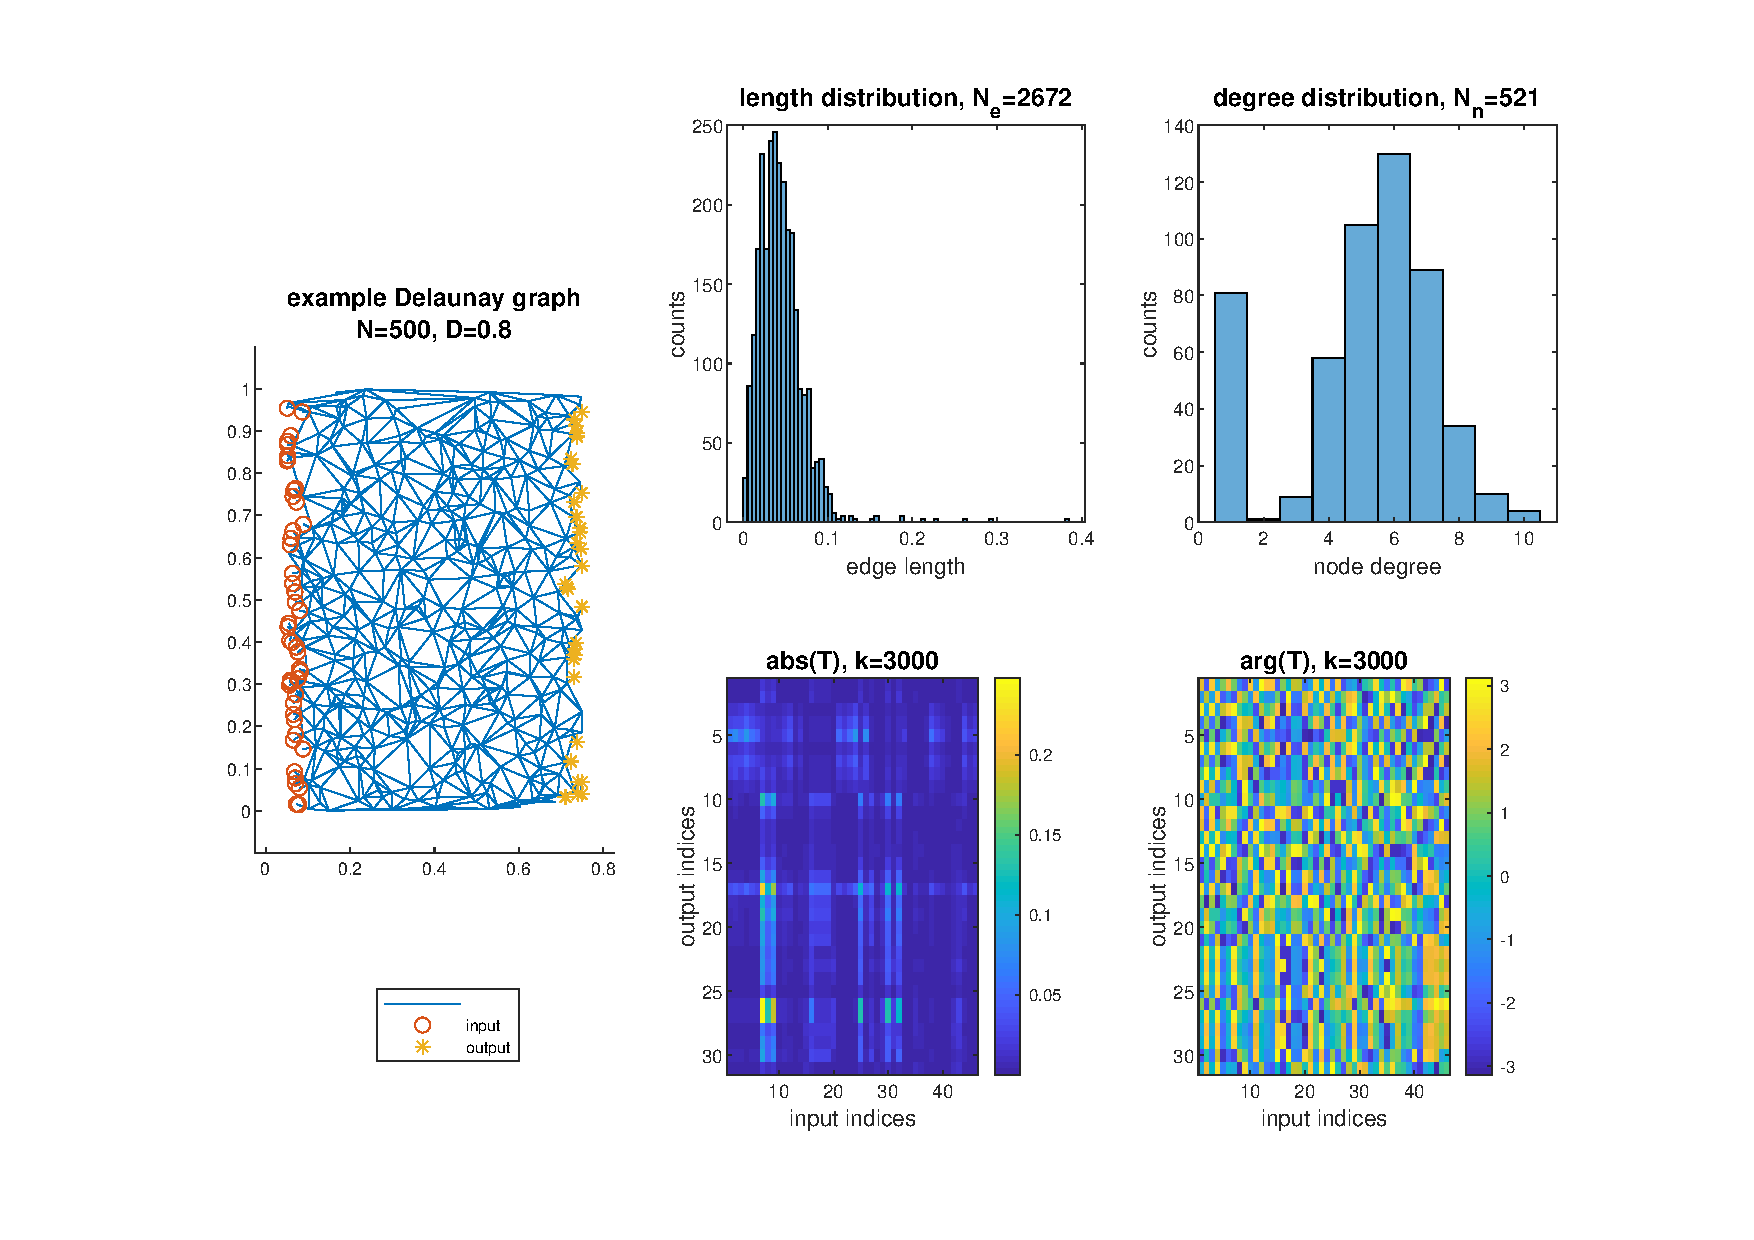
\includegraphics[width=\textwidth]{ch3/fig3/example_d.pdf}
    \caption{An example Delaunay graph. As a reminder, $N$ is the number of seed points, $D$ is the depth (width) of the graph, $N_e$ is the number of edges, $N_n$ is the number of nodes. Here $N_n \neq N$ because we have opened the graph on the left and right sides and added external nodes. The two plots in the bottom-right show the transmission matrix $T$ for $k=3000$: we see that $abs(T)$ which corresponds to transmitted intensity is sparse, while the output phase $arg(T)$ is fully randomised across $[-\pi,\pi]$.} 
    \label{fig:example_delaunay}
\end{figure}

\begin{figure}[h]
  \centering
    \includegraphics[width=\textwidth]{ch3/fig3/example_v.pdf}
    \caption{Same analysis as above, but for a Voronoi graph of different size. Here the discrepancy between $N_n$ and $N$ is larger due to the way in which Voronoi graphs are generated.} 
    \label{fig:example_voronoi}
\end{figure}

We will again start by analysing the behaviour of classical electromagnetic waves, and then adapt the simulation to quantum light.

\section{Scaling theory and localisation}
In the previous chapter we have constructed a bottom-up picture of the complex networks. To study multiple scattering and localisation properties, we need to take a top-down, statistical approach. There are several ways to characterise the localisation regime of a disordered system; the one we will focus on is scaling theory \cite{Muller2011,Abrahams1979}.

A short note on dimensionality is necessary before we proceed. Up until this point the networks have been described as 2D systems since they are planar graphs. However, although embedded in 2D space, they are not necessarily equivalent to 2D disordered systems in the context of multiple scattering.  





-mention coupled-dipole approximation \cite{Yurkin2007}


\section{Transmission and response modes}

\section{Boson sampling and quantum interference}

\section{Tuning and Loss}